\chapter{Indledning}
\section{Projektformulering}
Mange ældre har i dag svært ved at åbne deres vinflaske, da de ikke har den fornødne styrke til selv at trække korkproppen ud af vinflasken. Derfor vil det være ideelt for dem, at have en løsning hvor åbningen af vinflaskerne bliver automatiseret.

For at få den optimale oplevelse ud af en vin, skal den åbnes rettidigt så den iltes før indtagelse. Iltningstiden kan variere fra vin til vin, og derfor kan mange uerfarne vindrikkere have svært ved at ilte deres vin korrekt. Mange glemmer at åbne vinen i god tid, og opnår derfor ikke den optimale oplevelse. Det kan derfor være ideelt, hvis denne proces også automatiseres.

\begin{figure}[H]
	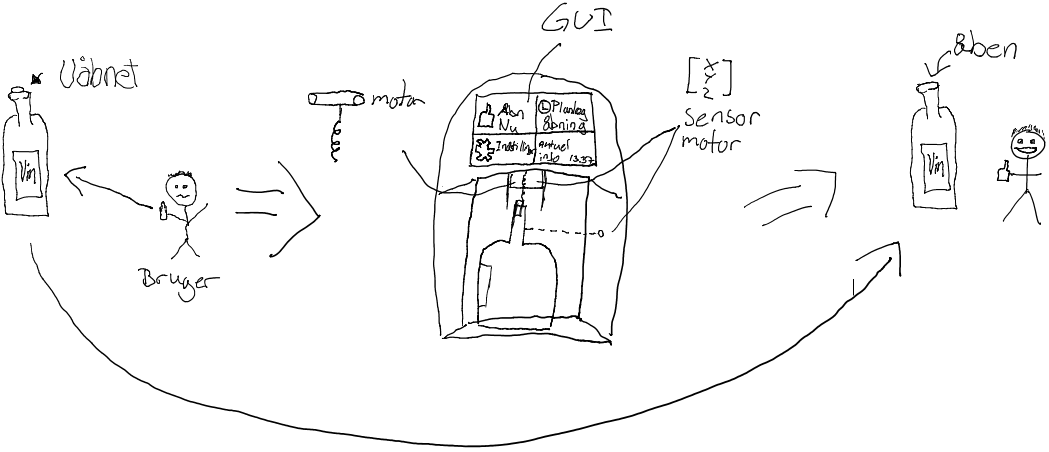
\includegraphics[scale=0.6]{WinePrep_realistisk.png}
	\caption{Rigt billede der beskriver WinePrep}
	\label{RIGTBILLEDE}
\end{figure}

\section{Det realistiske system}
WinePrep er den automatiske vinåbner som er illustreret på Figur \ref{RIGTBILLEDE}, hvilket beskriver det realistiske system i en tænkt situation. Der er siden udarbejdelsen af det rige billede ikke ændret ved tanken bag systemets funktionalitet, blot andre måder at implementere ideerne på.\\

Den oprindelige tanke med WinePrep gør det for brugeren muligt at åbne en bestemt type vinflaske ved at indsætte vinen i maskinen, konfigurere WinePrep til at åbne og derefter først lade systemet lokalisere flasken hvorefter en åbningsmekanisme sænker sig over vinen og trækker korkproppen op. Dette realiseres med WinePreps ramme, brugergrænseflade, sensorer, aktuatorer og proptrækker samt microcontrollere til at lade systemet kommunikere internt.

På baggrund af de tekniske komponenter og WinePreps kompleksitet, vil der til udviklere være krav om forhåndskendskab til elektronik og programmering, på et plan der gør det muligt at forstå og bruge de oplysninger der findes i bilagene til denne rapport.

WinePrep er en prototype der er mulig at udvikle og optimere på.

\section{Hovedansvarsområder}
Tabel xx viser fordelingen af hovedansvarsområder for produktet fordelt på gruppemedlemmer. Emnerne er inddelt i primær og sekundær, som informerer om medlemmers specialistviden og kernekompetencer indenfor produktudviklingen. Enkelte sekundære felter er tomme, dette betyder at ingen har været sekundær på emnet.\\

\begin{tabular}{| l | c | c |}
\hline
Emne & Primær & Sekundær\\\hline
Brugergrænseflade (GUI) & AS & HVB\\\hline
SPI DevKit-PSoC & HVB & JMH\\\hline
SPI PSoC-PSoC & HVB, JMH & \\\hline
PSoC software sensor & JMH & MBE\\\hline
PSoC software sensor & JMH & MBE\\\hline
Bipolære motorer & MBE & JMH\\\hline
Unipolære motorer & MBE & JMH\\\hline
DC motor & MBE & \\\hline
Konstruktion og mekanik & AS & HVB\\\hline
\end{tabular}